\documentclass{article}
\usepackage{amsmath}
\usepackage{algorithm2e}
\usepackage{graphicx}
\usepackage{cite}
\usepackage{url}
\usepackage{listings}
\usepackage{float,subcaption}
\usepackage{amsmath}
\usepackage{tikz}
\graphicspath{{images/}}

\begin{document}
	\title{A survey of adversarial attacks and robust learning on Deep Neural Networks}
	\maketitle
	
\section{Introduction}
Deep neural networks(DNNs) has proven to be quite efficacious in machine learning tasks, with recent adoption in automation systems and cyberphysical systems. Deep learning based on artificial neural networks is a very popular approach to modeling, classifying, and recognizing
complex data such as images, speech, and text. The unprecedented accuracy of deep learning methods has turned them into the foundation of new AI-based services on the Internet.
While the utility of deep learning is undeniable, the same
training data that has made it so successful also presents serious privacy issues. Centralized collection of photos,
speech, and video from millions of individuals is ripe with privacy risks; direct access to sensitive information.

With increasing popularity, security threats follow. Adversaries subtly alter legitimate
inputs (call input perturbation) to induce the trained model to produce erroneous outputs.
Adversarial samples can be used to, for
example, subvert fraud detection, bypass content filters or malware detection, or to mislead autonomous navigation systems. Adversarial sample transferability is the property that some adversarial samples produced to mislead a specific model F can mislead other models - even if their architectures greatly differ. A practical impact of this property is that it leads to black box attacks. 

\section{Related Works}
In \cite{szegedy2013intriguing}, it was discovered that several machine learning models including DNNs are vulnerable to adversarial samples. The cause of
these adversarial examples was a mystery, and speculative explanations have suggested it is due to extreme nonlinearity of deep
neural networks, perhaps combined with insufficient model averaging and insufficient regularization of the purely supervised
learning problem until then. \cite{szegedy2013intriguing} explained the existence of adversarial examples in linear models and linear perturbation in non-linear models and enabled a fast way of generating adversarial samples. 
\cite{goodfellow2014explaining} explained that the  primary cause of neural networks’ vulnerability to ad-
versarial perturbation is their linear nature. It also provides a detailed analysis with supportive experiments of adversarial training of linear models and the aspect of generalization of adversarial examples addressed in \cite{papernot2016transferability}.
\cite{hitaj2017deep} show that a distributed, federated,
or decentralized deep learning approach is fundamentally broken
and does not protect the training sets of honest participants. The
attack we developed exploits the real-time nature of the learning
process that allows the adversary to train a Generative Adversarial
Network (GAN) that generates prototypical samples of the targeted
training set that was meant to be private.
\cite{abadi2016deep} introduces the concept of distributed deep learning as a way to protect the privacy
of training data. In this model, multiple entities collaboratively train a model by sharing gradients of their individual
models with each other through a parameter server.

\section{Adversarial Training}
\cite{wang2016learning} propose a general framework to facilitate the development of adversary resistant DNNs.
	\subsection{Deep Neural Networks}
	\begin{figure}[h!]
		\centering
		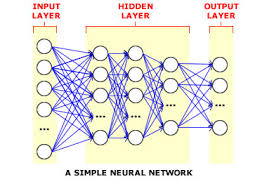
\includegraphics[width=0.9\columnwidth]{dnn}
		\caption{Neural Network Architecture}
		\label{fig:dnn}
	\end{figure}
	A typical DNN architecture, graphically depicted in \figurename{dnn}, consists of multiple successive
	layers of processing elements, or so-called “neurons”. Each processing layer can be viewed
	as learning a different, more abstract representation of the original multidimensional input
	distribution. As a whole, a DNN can be viewed as a highly complex function that is capable
	of nonlinearly mapping original high-dimensional data points to a lower dimensional space.
	Starting from the input, computing the activations of each subsequent layer simply requires,
	at minimum, a matrix multiplication usually followed by summation with a bias vector.
	This process roughly models the process of a layer of neurons integrating the information
	received from the layer below (i.e., computing a pre-activation) before applying an
	elementwise activation function.
	
	During the learning phase of the model, the DNN’s predictions are evaluated by comparing them with known target labels associated
	with the training samples (also known as the“ground truth”). Specifically, both predictions and labels are taken as the input to a
	selected cost function, such as cross-entropy. The DNN’s parameters are then optimized with respect to this cost function using the
	method of steepest gradient descent, minimizing prediction errors on the training set. Parameter gradients are calculated using back-
	propagation of errors. Since the gradients of the weights represent their influence on the final cost, there have been multiple
	algorithms developed for finding optimal weights more accurately and efficiently.
	More formally, given a training set (X, Y):
	{(x\textsubscript{1}, y\textsubscript{1}), (x\textsubscript{2}, y\textsubscript{2}), ...,(x\textsubscript{n}, y\textsubscript{n})}, where $x_i \epsilon R^m$ is a data sample and $y_i \epsilon R^k$ is data label, where, if categorical, is typically
	represented through a 1-of-k encoding. A standard neural network with a softmax output layer can be represented by the following
	function:
	\begin{equation}
		f : R\textsuperscript{m} \rightarrow R\textsuperscript{k}
	\end{equation}
	\begin{equation*}
		x \rightarrow f(x) 
	\end{equation*}
	The cost function for training a DNN as a (k-class) classifier is also defined as follows:
	\begin{equation}
	L : R\textsuperscript{m} \times R\textsuperscript{k} \rightarrow R
	\end{equation}
	\begin{equation*}
	f(x) \times y \rightarrow L(f(x), y) 
	\end{equation*}
	
	\subsection{Generating adversarial samples}
	Adversarial samples are generated by computing the derivative of the cost function with respect to the network’s input variables. The
	gradient of any input sample represents a direction vector in the model’s high-dimensional input space. Along this direction, a small
	change in this input sample can cause the DNN to generate a completely different prediction result. This particular direction is
	important since it represents the most effective way one might compromise the optimization of the cost function. Discovering this
	particular direction is realized by transmitting the error gradients from output layer all the way back to the input layer via back-
	propagation. The gradient with respect to the input may then be applied to the input sample(s) to craft an adversarial example(s).
	We now formally present the generation of adversarial samples by first defining the function g for generating any adversarial sample $\hat{x}$:
		\begin{equation}
		g : R\textsuperscript{m} \times R\textsuperscript{k} \rightarrow R\textsuperscript{m}
		\end{equation}
		\begin{equation*}
		x \times y \rightarrow \hat{x} 
		\end{equation*} 
		where
		\begin{equation}\label{4}
		\hat{x} = arg \ max \ L(f(\hat{x}), y) \ s.t \ ||\hat{x}-x||_p < \epsilon
		\end{equation} and $||.||_p$ is p-norm.
	
	Note that g is a one-to-one mapping, meaning that when there exist multiple x̂ satisfying \eqref{4}, only one is chosen. It should be noted that the constraint in \eqref{4} ensures that the distortion incurred by manipulation must be maintained at a small scale. Otherwise a significant distortion will leave the manipulation to be easily detected. Existing attacks \cite{carlini2017towards}, \cite{szegedy2013intriguing}, \cite{papernot2016limitations} consist of different approaches for generating adversarial samples which ultimately, can all be described solving following optimization problem, which is a transformation of \eqref{4}:
	\begin{equation}\label{5}
		\hat{x}: min c*||x - \hat{x}||_p - L(f(\hat{x}), y)
	\end{equation} 
	where c is some weight or coefficient. Here we refer to this type of attack as an optimal attack, and, for simplicity, denote $||x − \hat{x}||_p$ as the $l_p$ distance.
	Solving \eqref{5} is done much like solving for the weight coefficients of a standard DNN. Simply put, an attacker can use back-propagation and either gradient descent \cite{szegedy2013intriguing} or L-BFGS \cite{carlini2017towards}. In order to conduct the calculation, one first computes 
	$\partial^n L(f(\hat{x}, y)) / \partial \hat{x}^n$ and then use it for manipulating legitimate samples x. Note that here n = 1 if we use a first-order optimization method like gradient descent, or n = 2 if we utilize a second-order method such as the Newton–Raphson method. Since gradient descent requires an iterative calculation, it can be computationally expensive when the number of adversarial samples to be generated is large. To mitigate this problem, \cite{szegedy2013intriguing} proposed the fast gradient sign method to approximate this iterative calculation where
	one could use a single step of gradient descent, as follows:
	\begin{equation}
		\hat{x} = x + \epsilon . sign(\nabla L(f(x), y))
	\end{equation}
	where $\epsilon$ is set to control the scale of the distortions applied. Optimal attacks can be generalized to fast gradient sign attacks by selecting the $l_\infty$ distance. In \cite{szegedy2013intriguing}, the authors study an equivalent optimization problem to \eqref{5} by setting p = 2. Another type of attack, as described in \cite{papernot2016limitations}, generates adversarial samples using a greedy approach to solve \eqref{5} and sets p = 0. More specifically, adversarial samples are crafted by iteratively perturbing one coordinate of x at a time. A coordinate is picked by determining by its influence on the final cost.
	
\section{Attacks}
\subsection{Model Inversion(MI) Attack}
\cite{wang2016learning} explains this attack.
 Once the network has been trained, the gradient can be used to adjust the weights of the network and obtain a reverse-engineered example for all represented classes in the network. For those classes that it did not have prior information, it would still be able to recover prototypical examples. This attack shows that any accurate deep learning machine, no matter how it has been trained, can leak information about the different classes that it can distinguish.
 \paragraph{Limitation}: Due to the rich structure of deep learning machines, the model inversion attack may recover only prototypical examples that have little resemblance to the actual data that defined that class. It may or may not be considered as an attack as it may construct wrong/meaningless information.
 \subsection{Generative Adversarial Attack(GAN)}: The GAN procedure pits a discriminative deep learning network
 against a generative deep learning network. The discriminative network is trained to distinguish between images from an original database and those generated by the GAN. The generative network is first initialized with random noise, and at each iteration, it is trained to mimic the images in the training set of the discriminative network. The procedure ends when the discriminative network is unable to distinguish between samples from the original database and the samples generated by the generative network.
 
 \subsection{Black Box and White box attacks}: There are two main research directions in the literature on adversarial attacks based on different assumptions about the adversarial knowledge of the target network. The first and the most common line of work; whitebox attacks assumes that the adversary has detailed knowledge of the network architecture and the parameters resulting from training (or access to the labeled training set). Using this information, an adversary constructs a perturbation for a given image. The most effective methods are gradient-based: a small perturbation is constructed based on the gradient of the network loss function w.r.t. the input image. Often, adding this small perturbation to the original image leads to a misclassification. In the second line of work; black-box attacks, an adversary has restricted knowledge about the network from being able to only observe the network’s output on some probed inputs. This attack strategy is based the idea of greedy local search, an iterative search procedure, where in each round a local neighborhood is used to refine the current image and in process optimizing some objective function that depends on the network output. In each round, the local search procedure generates an implicit approximation to the actual gradient w.r.t the current image by observing changes in output. This approximate gradient provides a partial understanding of the influential pixels in the current image for the output, which is then used to update this image. 
 
 Note: Different examples to be added from \cite{rosenberg2017generic}
 
\subsection{Membership Inference Attack}:
To be added from \cite{shokri2017membership}

\subsection{Gray Box Attacks}
To be added from \cite{moosavi2016deepfool}

\bibliographystyle{unsrt}
\bibliography{ref_ml}

\end{document}
